
%(BEGIN_QUESTION)
% Copyright 2007, Tony R. Kuphaldt, released under the Creative Commons Attribution License (v 1.0)
% This means you may do almost anything with this work of mine, so long as you give me proper credit

Shown here is a pair of loop-powered 4-20 mA process transmitters, a process controller with dual measurement inputs, a 4-20 mA I/P (current-to-pressure) converter used to drive a pneumatically-actuated control valve, and a DAQ (data acquisition) unit for interfacing to a computer.  Both the process controller and DAQ unit inputs are ranged from 1 to 5 volts DC, not 4-20 mA:

$$\includegraphics[width=15.5cm]{i02274x01.eps}$$

Show how all three field devices would properly connect to the controller and to the DAQ unit at the same time, including the placement of resistors to convert the current signals into voltage signals that both the controller and the DAQ may interpret.

\vskip 20pt \vbox{\hrule \hbox{\strut \vrule{} {\bf Suggestions for Socratic discussion} \vrule} \hrule}

\begin{itemize}
\item{} A problem-solving technique useful for making proper connections in pictorial circuit diagrams is to first identify the directions of all DC currents entering and exiting component terminals, as well as the respective voltage polarity marks (+,$-$) for those terminals, based on your knowledge of each component acting either as an electrical {\it source} or an electrical {\it load}.  Discuss and compare how these arrows and polarity marks simplify the task of properly connecting wires between components. 
\item{} After you have sketched your circuit, evaluate the effects of various components failing either open or shorted, one at a time.
\end{itemize}

\underbar{file i02274}
%(END_QUESTION)





%(BEGIN_ANSWER)

\noindent
{\bf Partial answer:}

$$\includegraphics[width=15.5cm]{i02274x03.eps}$$

Note that shielded cables and shield grounds are omitted from this diagram for the same of simplicity.

%(END_ANSWER)





%(BEGIN_NOTES)

$$\includegraphics[width=15.5cm]{i02274x02.eps}$$

One important detail is that the DAQ ``Common'' terminal must be made common to the ``Ground'' terminal of the controller, in order to measure all three signals successfully.

%INDEX% Basics, 2-wire loop-powered transmitter: connection to process controller
%INDEX% Pictorial circuit review (4-20 mA loop)

%(END_NOTES)


